\section{Introduction}
The diffusion models (DMs) are powerful generative models that have demonstrated impressive performance \cite{ho2020denoising, song2020denoising, song2020score, dhariwal2021diffusion, nichol2021improved}. 
DMs have shown remarkable applications, including text-to-image synthesis \cite{ramesh2022hierarchical, rombach2022high, balaji2022ediffi, nichol2021glide}, inverse problems \cite{chung2022improving, lugmayr2022repaint}, and image editing \cite{hertz2022prompt, tumanyan2022plug, parmar2023zero, mokady2022null}.

% Diffusion models (DMs) are highly powerful generative models that have shown great performance \cite{ho2020denoising,song2020denoising,song2020score,dhariwal2021diffusion,nichol2021improved}.
% \yh{Instead of understanding the semantic structure of latent space itself,} 
% To control the generative process,
% existing methods have introduced conditional DMs, especially for text-to-image synthesis \cite{ramesh2022hierarchical,rombach2022high,balaji2022ediffi,nichol2021glide}, or mixing the latent variables $\vx_t$ of different sampling processes \cite{choi2021ilvr,meng2021sdedit,avrahami2022blended,liew2022magicmix,kawar2022imagic,avrahami2022spatext}.

Despite their achievements, the research community lacks a comprehensive understanding of the latent space of DMs and its influence on the generated results. So far, the completely diffused images are considered as latent variables but it does not have useful properties for controlling the results. For example, traversing along a direction from a latent produces weird changes in the results.
Fortunately, \citet{kwon2022diffusion} consider the intermediate feature space of the diffusion kernel, referred to as \ehspace{}, as a semantic latent space and show its usefulness on controlling generated images. In the similar sense, some works investigate the feature maps of the self-attention or cross-attention operations for controlling the results \cite{hertz2022prompt, tumanyan2022plug, parmar2023zero}, improving sample quality \cite{chefer2023attend}, or downstream tasks such as semantic segmentation \cite{ma2023diffusionseg, xu2023open}.
% They pair this with an asymmetric sampling process and
% They demonstrated that \ehspace{} possesses a linear semantic structure.
% Following the work of \citet{kwon2022diffusion}, there have been several analyses of the DM's feature space. These investigations explore the attention map and cross-attention map, which have been used for image editing \cite{hertz2022prompt, tumanyan2022plug, parmar2023zero} or improving sample quality \cite{chefer2023attend}. Moreover, these findings can be applied to downstream tasks such as segmentation using the feature space \cite{ma2023diffusionseg, xu2023open}.

% However, they rely solely on a proxy, $\mathbf{h}$, and do not directly deal with the latent variables $\vx_t$. 
% Furthermore, due to Kwon et al.'s modification of the internal feature of UNet, particularly where skip connections exist, there is no guarantee that significant changes will result in output quality. It is worth noting that the latent space \exspace{} is a sparse manifold, which makes meaningful editing within it challenging. Nevertheless, since \ehspace{} is clearly the codomain of \exspace{}, and given the fact that a meaningful semantic direction can be found in \ehspace{}, we can also define a semantic subspace in \exspace{}.

Still, the structure of the space $\mathcal{X}_t$ where latent variables $\{\vx_t\}$ live remains unexplored despite its crucial role in understanding DMs. It is especially challenging because 1) the model is trained to estimate the forward noise which does not depend on the input, as opposed to other typical supervisions such as classification or similarity, and 2) there are lots of latent variables over multiple recursive timesteps.
% Although the feature space has been thoroughly explored, the latent space $\vx{}_t \in \mathcal{X}$ remains unexplored despite its crucial role in understanding DMs.
% This is due to the fact that the latent variable of DM, $\vx{}_t$, consists primarily of noised images.
% Therefore, it is not reasonable to expect any significant semantic structure in the latent space \exspace{}.
% \yh{Another reason is the the characteristic iterative process of the DMs which involves a sequence of noisy images and subtle noises, i.e., the embeddings are not directly connected to the final images.}
In this paper, we aim to analyze \exspace{} in conjunction with its corresponding representation \ehspace{}, by incorporating a local geometry to \exspace{} using the concept of a {\it pullback metric} in Riemannian geometry. 
% Our paper contributes:

\begin{figure}[!t]
    \centering
    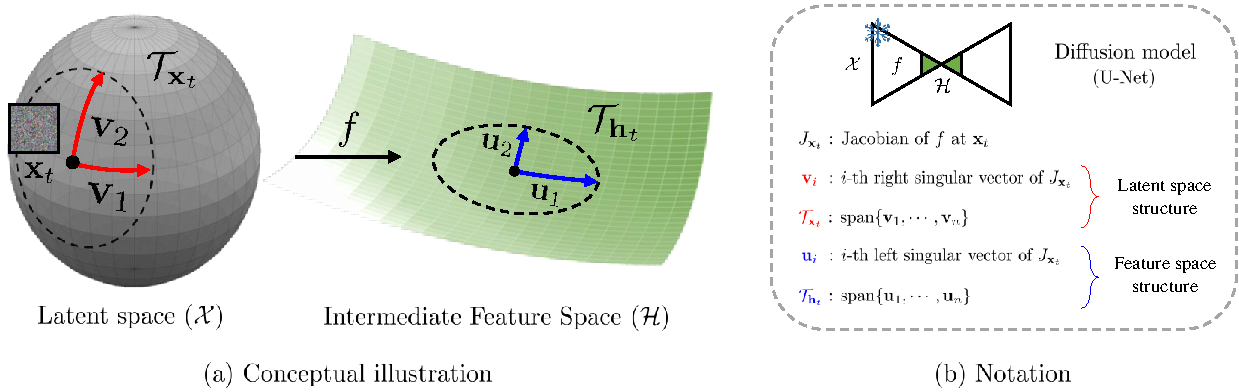
\includegraphics[width=1\linewidth]{figure/teaser_rebuttal_3.pdf}
    \caption{\textbf{Conceptual illustration of local geometric structure.} 
    (a) The local basis $\{\mathbf{v}_1, \mathbf{v}_2, \cdots \}$ of the local latent subspace $\mathcal{T}_{{\mathbf{x}}_t}$ within the latent space $\mathcal{X}$ is interlinked with the local basis $\{\mathbf{u}_1, \mathbf{u}_2, \cdots\}$ of the local tangent space $\mathcal{T}_{{\mathbf{h}}_t}$ in the feature space $\mathcal{H}$.
    % (b) The derivation of these local bases is facilitated through the singular value decomposition (SVD) of the Jacobian originating from the U-Net responsible for encoding the feature map $f$, which connects $\mathcal{X}$ and $\mathcal{H}$.
    (b) The derivation of these local bases is facilitated through the singular value decomposition (SVD) of the Jacobian, which emanates from the U-Net responsible for encoding the feature map \(f\), linking \(\mathcal{X}\) and \(\mathcal{H}\).
    }
    \vspace{-1em}
    \label{fig:teaser}
\end{figure}

% \begin{figure}[!t]
%     \centering
%     % 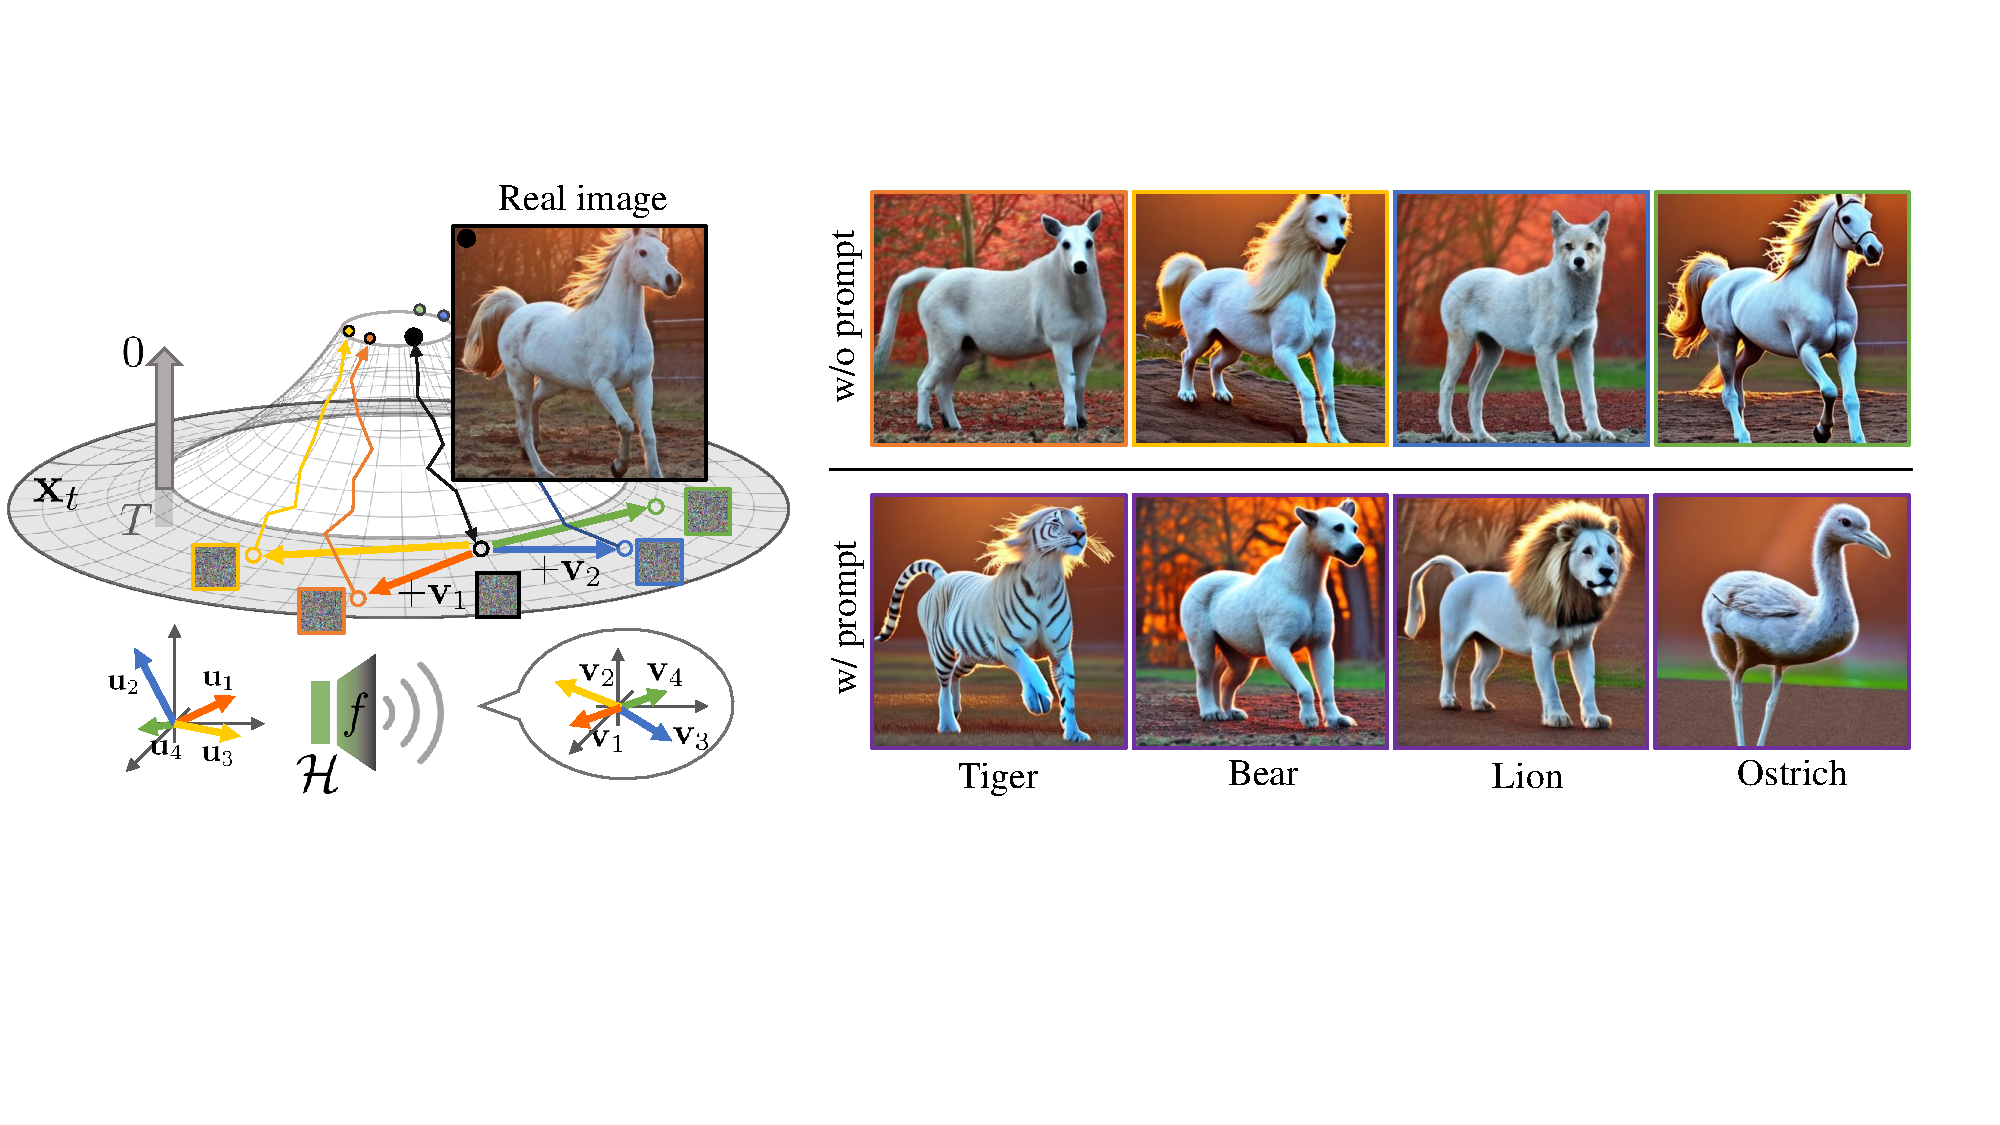
\includegraphics[width=1\linewidth]{figure/teaser_new.pdf}
%     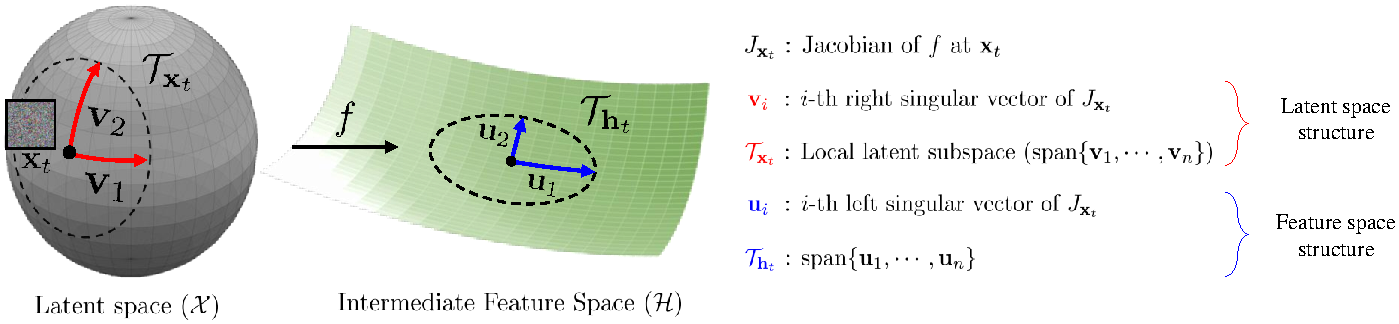
\includegraphics[width=1\linewidth]{figure/teaser_rebuttal.pdf}
%     \caption{\textbf{Conceptual illustration of our method.} 
%     % We employ an unsupervised approach to discover latent basis vectors in the latent space $\vx_t$, leveraging the Riemannian geometry between $\vx_t$ and $\vh_t$. Here, $\mathcal{H}$ represents the bottleneck layer, and $f$ denotes the frozen encoder of a U-Net. 
%     % The identified directions allow for the manipulation of the semantic content in the generated images. Text conditioning with prompts can be also used for targeted image editing.
%     We employ an unsupervised approach to discover the latent basis in the latent space $\mathcal{X}_t$.
%     }
%     \vspace{-1em}
%     \label{fig:teaser}
% \end{figure}

First, we discover the local latent basis for \exspace{} and the corresponding local tangent basis for \ehspace{}.
The local basis is obtained by performing singular value decomposition (SVD) of the Jacobian of the mapping from \exspace{} to \ehspace{}.
To validate the discovered local latent basis, we demonstrate that 
walking along the basis
% \yh{traversal along the basis} 
can edit real images in a semantically meaningful way. 
Furthermore, we can use the discovered local latent basis vector to edit other samples by using parallel transport, when they exhibit comparable local geometric structures.
Note that existing editing methods manipulate the self-attention map or cross-attention map over multiple timesteps \cite{hertz2022prompt, tumanyan2022plug, parmar2023zero}. On the other hand, we manipulate only $\vx_t$ once at a specific timestep.

Second, we investigate how the latent structures differ across different timesteps and samples as follows.
% Second, we investigate how the semantic structure changes over time and \jo{between samples}. %identified two trends.
The frequency domain of the local latent basis shifts from low-frequency to high-frequency along the generative process. 
% Although this was observed indirectly in a previous study by \citet{choi2022perception},
We explicitly confirm it using power spectral density analysis.
The difference between local tangent spaces of different samples becomes larger along the generative process. 
The local tangent spaces at various diffusion timesteps are similar to each other if the model is trained on aligned datasets such as CelebA-HQ or Flowers. However, this homogeneity does not occur on complex datasets such as ImageNet.

% We compared the evolution of the local tangent basis over time and identified groups of timesteps exhibiting with similar semantic structures. 
% Within each group, DMs processed similar basis, even when given different timesteps.
% TODO ImageNet 에서의 양상 확인
% gDDIM 의 denoising process 를 나누는 기준을 떠올리게 한다. 
% TODO
% 이 관찰으로부터 유사한 semantic structure 를 갖는 구간을 clustering 하고, 각 cluster 에서 redundant 하지 않은 timestep scheduling 을 제안하고 sampling quality 를 개선했다.

Finally, we examine how the prompts affect the latent structure of text-to-image DMs as follows.
Similar prompts yield similar latent structures. Specifically, we find a positive correlation between the similarity of prompts and the similarity of local tangent spaces.
The influence of text on the local tangent space becomes weaker along the generative process. %, specifically when the diffusion timestep is $t<0.7T$. $T$ is the maximum length of a diffusion process.
%\textcircled{\raisebox{-0.9pt}{1}} 
%\textcircled{\raisebox{-0.9pt}{2}} 

% \modify{With ChatGPT LOL :) 고쳐야함.ㅋㅋ}
% 우리의 연구는 지금까지 탐구되지 않았던 DM x 에 대한 
% Our research uncovers the hidden depths of the latent space \exspace{} within DMs, revealing a profound understanding and intuition that has remained elusive. This newfound knowledge not only empowers us to achieve real image editing through unsupervised methods but also offers a glimpse into the underlying principles of generative models, opening up a realm of endless possibilities and uncharted territories. % 

{
% Our work examines the geometric structure of \exspace{} and \ehspace{} via Riemannian geometry. 
% As a result, we discover the latent structure of \exspace{}, and how the geometric structure evolves along a generative process and is affected by prompts. 
% This geometrical perspective deepen our understanding of DMs.
% Our work examines the geometry of \exspace{} and \ehspace{} through Riemannian geometry. As a result, we discover the latent structure of \exspace{} and how the geometric structure evolves along a generative process and is affected by prompts. 
% Our exploration from a geometrical perspective deepens our understanding of DMs.
Our work examines the geometry of \exspace{} and \ehspace{} using Riemannian geometry. We discover the latent structure of \exspace{} and how it evolves during the generative process and is influenced by prompts. This geometric exploration deepens our understanding of DMs.
}

% In the experiments, we demonstrate that the directions found in an unsupervised manner indeed lead to semantic changes in the images. 
% We note that discovering the editing directions in the latent variables of diffusion models has not been tackled.
% \mingi{}
% Furthermore, we provide thorough quantitative and qualitative analyses on the aforementioned properties. Our method even works on stable diffusion \cite{rombach2022high}.